\documentclass[]{article}
\usepackage{lmodern}
\usepackage{amssymb,amsmath}
\usepackage{ifxetex,ifluatex}
\usepackage{fixltx2e} % provides \textsubscript
\ifnum 0\ifxetex 1\fi\ifluatex 1\fi=0 % if pdftex
  \usepackage[T1]{fontenc}
  \usepackage[utf8]{inputenc}
\else % if luatex or xelatex
  \ifxetex
    \usepackage{mathspec}
  \else
    \usepackage{fontspec}
  \fi
  \defaultfontfeatures{Ligatures=TeX,Scale=MatchLowercase}
\fi
% use upquote if available, for straight quotes in verbatim environments
\IfFileExists{upquote.sty}{\usepackage{upquote}}{}
% use microtype if available
\IfFileExists{microtype.sty}{%
\usepackage[]{microtype}
\UseMicrotypeSet[protrusion]{basicmath} % disable protrusion for tt fonts
}{}
\PassOptionsToPackage{hyphens}{url} % url is loaded by hyperref
\usepackage[unicode=true]{hyperref}
\hypersetup{
            pdfborder={0 0 0},
            breaklinks=true}
\urlstyle{same}  % don't use monospace font for urls
\usepackage{graphicx,grffile}
\makeatletter
\def\maxwidth{\ifdim\Gin@nat@width>\linewidth\linewidth\else\Gin@nat@width\fi}
\def\maxheight{\ifdim\Gin@nat@height>\textheight\textheight\else\Gin@nat@height\fi}
\makeatother
% Scale images if necessary, so that they will not overflow the page
% margins by default, and it is still possible to overwrite the defaults
% using explicit options in \includegraphics[width, height, ...]{}
\setkeys{Gin}{width=\maxwidth,height=\maxheight,keepaspectratio}
\IfFileExists{parskip.sty}{%
\usepackage{parskip}
}{% else
\setlength{\parindent}{0pt}
\setlength{\parskip}{6pt plus 2pt minus 1pt}
}
\setlength{\emergencystretch}{3em}  % prevent overfull lines
\providecommand{\tightlist}{%
  \setlength{\itemsep}{0pt}\setlength{\parskip}{0pt}}
\setcounter{secnumdepth}{0}
% Redefines (sub)paragraphs to behave more like sections
\ifx\paragraph\undefined\else
\let\oldparagraph\paragraph
\renewcommand{\paragraph}[1]{\oldparagraph{#1}\mbox{}}
\fi
\ifx\subparagraph\undefined\else
\let\oldsubparagraph\subparagraph
\renewcommand{\subparagraph}[1]{\oldsubparagraph{#1}\mbox{}}
\fi

% set default figure placement to htbp
\makeatletter
\def\fps@figure{htbp}
\makeatother


\date{}

\begin{document}

\subsection{UGA : TER 2020-21 : Majeur
Mathématiques}\label{uga-ter-2020-21-majeur-mathuxe9matiques}

\subsection{Titre : Loi de réciprocité
quadratique}\label{titre-loi-de-ruxe9ciprocituxe9-quadratique}

Résumé : en théorie des nombres, la loi de réciprocité quadratique,
établit des liens entre les nombres premiers ; plus précisément, elle
décrit la possibilité d'exprimer un nombre premier comme un carré modulo
un autre nombre premier. Conjecturée par Euler et reformulée par
Legendre, elle a été correctement démontrée pour la première fois par
Gauss en 1801. Elle permet de résoudre les deux problèmes de base de la
théorie des résidus quadratiques et est considérée comme un des
théorèmes les plus importants de la théorie des nombres, ayant de
nombreuses généralisations.

\textbf{Théorème fondamental}

Étant donnés deux nombres premiers impairs distincts p et q :

\begin{itemize}
\tightlist
\item
  si p ou q est congru à 1 modulo 4, alors p est un carré modulo q si et
  seulement si q est un carré modulo p.
\item
  si p et q sont congrus à 3 modulo 4, alors p est un carré modulo q si
  et seulement si q n'est pas un carré modulo.
\end{itemize}

Les premières démonstrations aujourd'hui considérées comme complètes
sont publiées par Gauss dans ses \emph{Disquisitiones arithmeticae} en
1801. On compte plus de 200 démonstrations et parmi elles la preuve de
D. Zagier est remarquable car elle ne tient qu'une ligne.

On va étudier trois preuves de ce résultat :

\begin{itemize}
\tightlist
\item
  à la base de la division euclidienne dans les entiers de Gauss.
\item
  en étudiant des modules libre de rang 2 suivant Lucas.
\item
  avec l'involution de Zagier et son interpretation en termes de la
  combinatoire des moulins à vents decouverte par A. Spivak.
\end{itemize}

En particulier, on mettra en avant la géométrie sous adjacente dans les
preuves.

\begin{figure}
\centering
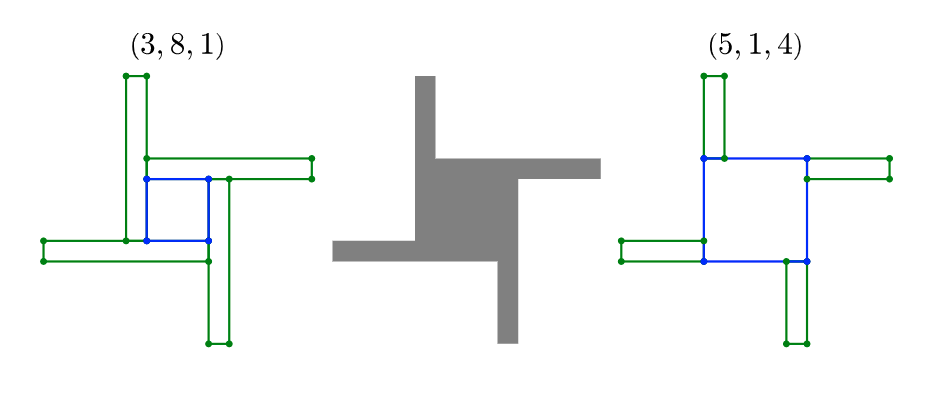
\includegraphics{./windmills.png}
\caption{img}
\end{figure}

\href{https://mathoverflow.net/questions/31113/zagiers-one-sentence-proof-of-a-theorem-of-fermat}{source}

\subsection{Prérequis :}\label{pruxe9requis}

Algèbre II

\subsection{Références}\label{ruxe9fuxe9rences}

\begin{enumerate}
\def\labelenumi{\arabic{enumi}.}
\item
  Christian Elsholtz, A combinatorial approach to sums of two squares
  and related problems
  \href{https://www.math.tugraz.at/~elsholtz/WWW/papers/papers30nathanson-new-address3.pdf}{télécharger}
\item
  Wagon, S.: The Euclidean algorithm strikes again. Amer. Math. Monthly
  97 (1990), 125--129.
\item
  Zagier, D.: A one-sentence proof that every prime p = 1 (mod 4) is a
  sum of two squares, Amer. Math. Monthly 97(2) (1990), 144. p
\end{enumerate}

\end{document}
